\documentclass[11pt,a4paper]{article}
\usepackage[utf8]{inputenc}
\usepackage[T1]{fontenc}
\usepackage{lmodern}
\usepackage[margin=1in]{geometry}
\usepackage{graphicx}
\usepackage{booktabs}
\usepackage{array}
\usepackage{longtable}
\usepackage{multirow}
\usepackage{makecell}
\usepackage{tabularx}
\usepackage{colortbl}
\usepackage{xcolor}
\usepackage{hyperref}
\usepackage{url}
\usepackage{amsmath}
\usepackage{amssymb}
\usepackage{enumitem}
\usepackage{caption}
\usepackage{subcaption}
\usepackage{float}
\usepackage{pgfplots}
\usepackage{tikz}
\usetikzlibrary{shapes.geometric, arrows, positioning, calc, fit, backgrounds}
\pgfplotsset{compat=1.17}
\usepackage{setspace}
\onehalfspacing

\hypersetup{
    colorlinks=true,
    linkcolor=blue,
    filecolor=magenta,
    urlcolor=blue,
    citecolor=blue
}
\definecolor{headerblue}{RGB}{31,78,120}
\definecolor{lightgray}{RGB}{240,240,240}
\title{\textbf{A Systematic Literature Review on Large Language Model-Based \\
Code Generation: Bug Taxonomy, Repair Techniques, and \\
Multi-Agent Collaborative Frameworks}}

\author{
Muhmmad Immad Ahmed Khan, Adan Shahzad, Zikria Akhtar, Mudassar Adeel  \\   
\small Capital University of Science and Technology, Islamabad, Pakistan \\
}
\date{\today}

\begin{document}

\maketitle

%====================================================================
% ABSTRACT
%====================================================================
\begin{abstract}
\noindent
 The rapid advancement of Large Language Models (LLMs) has transformed automated code generation, yet LLM-generated code continues to exhibit syntactic errors, runtime failures, functional bugs, and security vulnerabilities. Despite significant research efforts addressing these issues in isolation, there is a lack of a systematic synthesis of contemporary techniques spanning code generation, bug detection, automated repair, optimization, and multi-agent collaboration.

\noindent
This Systematic Literature Review (SLR) aims to identify, classify, and analyze the latest research practices (2021--2025) where LLM-based approaches have been utilized for code generation, bug taxonomy construction, automated program repair, efficiency optimization, and security assurance. The review further investigates the tools, frameworks, and benchmarks employed, and highlights research gaps that motivate the development of Multi-Agent Collaborative Intelligence (MACI) systems.

\noindent
 Systematic Literature Review methodology has been adopted following the guidelines proposed by Kitchenham. A comprehensive review protocol was developed incorporating six concrete selection criteria, a structured search process across four renowned scientific databases (IEEE, ACM, Springer, Elsevier, supplemented by arXiv), quality assessment procedures, and a formal data extraction and synthesis framework. The six predefined categories guided the classification of selected research works.

\noindent
 From an initial pool of 4{,}287 candidate studies, 24 primary research works were selected through a rigorous multi-stage filtering process. The selected studies were classified into six categories: General, Code Generation, Bug Detection \& Classification, Code Repair, Code Optimization, and Security. The analysis identified Chain-of-Thought (CoT) and its structured variants as the most frequently employed prompting techniques (used in 58.3\% of studies), self-critique with compiler feedback as the dominant repair strategy (45.8\%), and HumanEval/MBPP/APPS as the most widely used benchmarks. A comprehensive comparative evaluation of 18 tools and frameworks was performed using both general and activity-specific characteristics.

\noindent
 The SLR reveals that contemporary LLM-based code generation research predominantly targets individual concerns (correctness, efficiency, or security) in isolation, with limited integration across the full software development lifecycle. A significant research gap exists in unified multi-agent frameworks that simultaneously address generation quality, bug detection, iterative repair, and security enforcement. This gap justifies the development of MACI-style collaborative systems that orchestrate specialized agents through structured communication and iterative refinement to produce correct, efficient, secure, and maintainable code.

\noindent
\textbf{Keywords:} Systematic Literature Review, Large Language Models, Code Generation, Bug Taxonomy, Automated Program Repair, Multi-Agent Systems, Chain-of-Thought Prompting
\end{abstract}

\newpage

%====================================================================
% SECTION 2.1 — LITERATURE REVIEW INTRODUCTION
%====================================================================
\section{Literature Review}
\label{sec:lit_review}

The emergence of Large Language Models (LLMs) such as GPT-4, Claude-3, DeepSeek-V3/R1, Code Llama, and StarCoder-2 has fundamentally reshaped the landscape of automated software engineering. Modern LLM-based code generation systems have achieved unprecedented levels of performance on standard benchmarks, with state-of-the-art models such as DeepSeek-R1 achieving up to 77.9\% pass rates on real-world programming tasks \cite{dou2026}. However, despite this remarkable progress, LLM-generated code continues to exhibit critical shortcomings, including syntax violations, runtime exceptions, functional bugs, inefficient algorithmic implementations, and security vulnerabilities \cite{bruni2025,liu2025llm4tdg}. Contemporary research has responded to these challenges through diverse technical strategies ranging from structured prompting and multi-agent orchestration to iterative self-repair and formal verification. Nevertheless, the fragmentation of this research landscape, with individual studies addressing narrow slices of the broader problem, motivates the need for a systematic synthesis. This Systematic Literature Review (SLR) consolidates and analyzes 24 primary studies published between 2021 and 2025, providing researchers and practitioners with an evidence-based foundation for future work in LLM-based code generation and collaborative agent-based frameworks.

%====================================================================
% SECTION 2.1.1 — BACKGROUND
%====================================================================
\subsection{Background}
\label{sec:background}

Code generation, historically framed as a program synthesis problem, aims to produce executable programs from high-level specifications such as natural language requirements or input-output examples \cite{chen2021humaneval,austin2021mbpp}. Early approaches relied on deductive synthesis and inductive programming, both of which required formally specified inputs and were limited to narrow domains. The introduction of the Transformer architecture and its subsequent scaling into Large Language Models catalyzed a paradigm shift: LLMs trained on massive corpora of source code can now translate informal natural language descriptions into syntactically and semantically plausible code through next-token prediction \cite{chen2021humaneval}.

Three foundational benchmarks established the evaluation landscape that shapes contemporary research: \textit{HumanEval} \cite{chen2021humaneval} with 164 hand-crafted Python problems, \textit{MBPP} \cite{austin2021mbpp} with 974 crowd-sourced entry-level problems, and \textit{APPS} \cite{hendrycks2021apps} with 10,000 competitive programming problems stratified by difficulty. These benchmarks introduced the \texttt{pass@k} metric as the de facto correctness criterion. However, recent research has documented that functional correctness alone is an insufficient measure of code quality: generated code may pass tests while harboring efficiency issues \cite{jonnala2025}, security vulnerabilities \cite{bruni2025,ding2025codingcare}, code smells \cite{zhang2024copilot}, or maintainability problems \cite{zhang2025anncoder}.

To address these multi-dimensional concerns, the research community has developed several complementary strategies. \textit{Prompt engineering} techniques, particularly Chain-of-Thought (CoT) \cite{wei2022cot} and Structured Chain-of-Thought (SCoT) \cite{li2025scot}, guide models through explicit reasoning steps before code synthesis. \textit{Multi-agent frameworks} such as ChatDev \cite{qian2023chatdev}, MetaGPT \cite{hong2023metagpt}, and AutoGen \cite{wu2023autogen} decompose software development tasks into role-specialized agents communicating through structured protocols. \textit{Automated program repair} techniques \cite{xia2023apr,chen2023selfdebug,wang2024intervenor} leverage LLMs' reasoning capabilities to identify and fix bugs iteratively using compiler feedback. \textit{Security-aware generation} frameworks such as PromSec \cite{nazzal2024promsec} and CodingCare \cite{ding2025codingcare} integrate vulnerability detection into the generation pipeline.

Notably, the recent work by Dou et al. \cite{dou2026} represents a significant milestone: it provides the first comprehensive empirical analysis of bugs in LLM-generated code, proposing a three-tier bug taxonomy (syntax, runtime, functional) with ten secondary categories, introducing a real-world benchmark (RWPB) to address data leakage concerns, and demonstrating a self-critique-based iterative repair mechanism. However, Dou et al.'s work primarily operates within a single-agent paradigm, leaving open the question of whether multi-agent collaborative frameworks can further improve the accuracy, efficiency, and security of LLM-generated code.

This SLR synthesizes the state of the art across these research threads, identifying the techniques, tools, and benchmarks that have proven most effective, and pinpointing the research gap that motivates the development of Multi-Agent Collaborative Intelligence (MACI) frameworks.

%====================================================================
% SECTION 2.1.2 — RESEARCH QUESTIONS
%====================================================================
\subsection{Research Questions}
\label{sec:research_questions}

Four research questions guide this SLR. These questions are designed to be precise and actionable, providing the analytical basis for the selection, classification, and synthesis of primary studies.

\begin{itemize}[leftmargin=*]
\item \textbf{RQ1:} What important researches have been reported from 2021 to 2025 where LLM-based approaches have been utilized to support code generation, bug detection, automated repair, efficiency optimization, and security assurance?

\item \textbf{RQ2:} Which prompting techniques (Zero-shot, Few-shot, Chain-of-Thought, Structured Chain-of-Thought, Self-Planning, Recursive Criticism and Improvement) are more frequently utilized for LLM-based code generation during 2021--2025 researches?

\item \textbf{RQ3:} Which bug detection and repair approaches (self-critique with compiler feedback, constraint-based reasoning, multi-agent collaboration, static analysis integration, evolutionary optimization) are more frequently utilized during 2021--2025 researches?

\item \textbf{RQ4:} What are the significant tools, frameworks, and benchmarks for code generation, bug detection, repair, optimization, and security in the context of LLM-based code generation, and how can they be compared based on general and activity-specific characteristics?
\end{itemize}

%====================================================================
% SECTION 2.1.3 — CATEGORIES DEFINITION
%====================================================================
\subsection{Categories Definition}
\label{sec:categories}

Six categories have been defined to systematically organize the selected research works. This categorization ensures accurate classification of primary studies and improves the precision of the answers to our research questions. The categories are mutually complementary; a study addressing multiple LLM-based code generation activities simultaneously is assigned to the \textit{General} category, whereas studies targeting a specific activity are assigned to the corresponding specialized category.

\subsubsection*{2.1.3.1 General Category}
This category contains research works where comprehensive solutions covering multiple LLM-based code generation activities (e.g., generation plus repair, or end-to-end pipelines spanning requirement analysis, code synthesis, review, and iterative refinement) are proposed. Studies covering at least three of the six activity types are assigned to this category.

\subsubsection*{2.1.3.2 Code Generation Category}
This category includes research works primarily focused on improving the generation of code from natural language specifications through techniques such as prompt engineering, in-context learning, planning-based decomposition, and structured reasoning. Such researches do not significantly contribute to bug repair, optimization, or security aspects.

\subsubsection*{2.1.3.3 Bug Detection and Classification Category}
This category encompasses research works that propose taxonomies, classification schemes, or detection methodologies for bugs introduced by LLM-generated code. These studies typically construct bug datasets, analyze root causes, and provide empirical insights into the limitations of contemporary LLMs.

\subsubsection*{2.1.3.4 Code Repair Category}
This category contains research works proposing automated program repair mechanisms specifically tailored for LLM-generated or LLM-augmented code. Techniques in this category include self-debugging, iterative refinement with compiler feedback, teacher-student repair frameworks, and formal verification-based repair.

\subsubsection*{2.1.3.5 Code Optimization Category}
This category includes research works addressing the efficiency, quality, readability, or maintainability of LLM-generated code. Techniques include evolutionary optimization, rule-based static analysis, candidate ranking, and fine-tuning for efficiency.

\subsubsection*{2.1.3.6 Security Category}
This category encompasses research works focused on the security dimension of LLM-generated code, including vulnerability detection, secure prompt engineering, CVE mitigation, and integration of security-aware knowledge bases into generation pipelines.

%====================================================================
% SECTION 2.1.4 — INCLUSION/EXCLUSION CRITERIA
%====================================================================
\subsection{Inclusion and Exclusion Criteria}
\label{sec:inclusion_criteria}

Six concrete parameters have been defined to ensure the correctness and relevance of the answers to our research questions. Each candidate research work is evaluated against these parameters.

\begin{enumerate}[leftmargin=*]
\item \textbf{Subject-relevant:} Select the research work only if it is relevant to our research context. It must support the answers of our research questions and must be relevant to one of the six predefined categories (Section~\ref{sec:categories}). Reject irrelevant researches that do not belong to any of the six predefined categories.

\item \textbf{2021--2025:} Selected research work must be published from 2021 to 2025. This ensures the inclusion of only the most recent advances in LLM-based code generation, coinciding with the emergence of large-scale code-capable LLMs (e.g., Codex, GPT-3.5/4, DeepSeek-Coder). Reject all researches published before 2021.

\item \textbf{Publisher:} Selected research work must be published in one of the four renowned scientific databases i.e., IEEE, Springer, Elsevier, ACM, or be a highly-cited preprint on arXiv that has subsequently been accepted at a top venue (e.g., NeurIPS, ICML, ICLR, ICSE, FSE, OOPSLA).

\item \textbf{Crucial-effects:} Selected research work must have crucial positive effects on LLM-based code generation, bug detection, repair, optimization, or security. Reject the research work if its proposal does not have significant consequences, as determined by experimental validation or theoretical contribution.

\item \textbf{Results-oriented:} Selected research work must be results-oriented. The proposal and ultimate outcomes of the research must be supported by solid facts and experimentation, with clear evaluation metrics (e.g., pass@k, bug reduction rate, security scanner output). Reject the research work if its proposal is verified through weak validation methods.

\item \textbf{Repetition:} All researches in a particular research context cannot be included. Consequently, reject researches that are identical in contribution and only retain the most representative and highly-cited work per research thread.
\end{enumerate}

%====================================================================
% SECTION 2.1.5 — SEARCH PROCESS
%====================================================================
\subsection{Search Process}
\label{sec:search_process}

The search process was systematically executed across four renowned scientific databases (IEEE Xplore, ACM Digital Library, SpringerLink, Elsevier ScienceDirect) and arXiv. A combination of search terms with AND/OR Boolean operators was employed, and the ``2021--2025'' publication filter was applied universally. Table~\ref{tab:search_terms} summarizes the search terms and the number of results obtained from each database.

\begin{table}[H]
\centering
\caption{Search terms with Boolean operators and number of search results per database.}
\label{tab:search_terms}
\small
\begin{tabular}{@{}clccccc@{}}
\toprule
\textbf{\#} & \textbf{Search Term} & \textbf{Operator} & \textbf{IEEE} & \textbf{Springer} & \textbf{Elsevier} & \textbf{ACM} \\
\midrule
1 & LLM code generation & AND & 487 & 632 & 298 & 521 \\
2 & Large language model code synthesis & AND & 312 & 421 & 189 & 387 \\
3 & Chain-of-thought code & AND & 156 & 203 & 112 & 241 \\
4 & Structured prompting code generation & AND & 89 & 132 & 78 & 156 \\
5 & Bug taxonomy LLM & AND & 47 & 89 & 62 & 103 \\
6 & Automated program repair LLM & OR & 342 & 478 & 251 & 419 \\
 & & AND & 124 & 187 & 96 & 172 \\
7 & Multi-agent code generation & AND & 98 & 167 & 82 & 143 \\
8 & Self-critique code repair & AND & 62 & 98 & 47 & 89 \\
9 & Secure code generation LLM & AND & 134 & 198 & 87 & 167 \\
10 & Code efficiency LLM optimization & AND & 76 & 121 & 68 & 109 \\
11 & HumanEval benchmark evaluation & AND & 203 & 178 & 94 & 234 \\
12 & MBPP APPS code benchmark & OR & 287 & 312 & 156 & 298 \\
 & & AND & 112 & 154 & 87 & 147 \\
13 & Static analysis code generation & AND & 167 & 243 & 132 & 198 \\
14 & Retrieval augmented code generation & AND & 89 & 143 & 76 & 124 \\
15 & Real-world benchmark data leakage & AND & 67 & 98 & 54 & 87 \\
\midrule
\multicolumn{3}{r}{\textbf{Total initial results:}} & \textbf{2{,}852} & \textbf{3{,}954} & \textbf{1{,}869} & \textbf{3{,}595} \\
\bottomrule
\end{tabular}
\end{table}

The filtering process followed a PRISMA-inspired multi-stage pipeline as depicted in Figure~\ref{fig:prisma}. Starting from 4{,}287 candidate studies (after removing cross-database duplicates), progressively stringent filters were applied to retain the final set of 24 primary studies.

\begin{figure}[H]
\centering
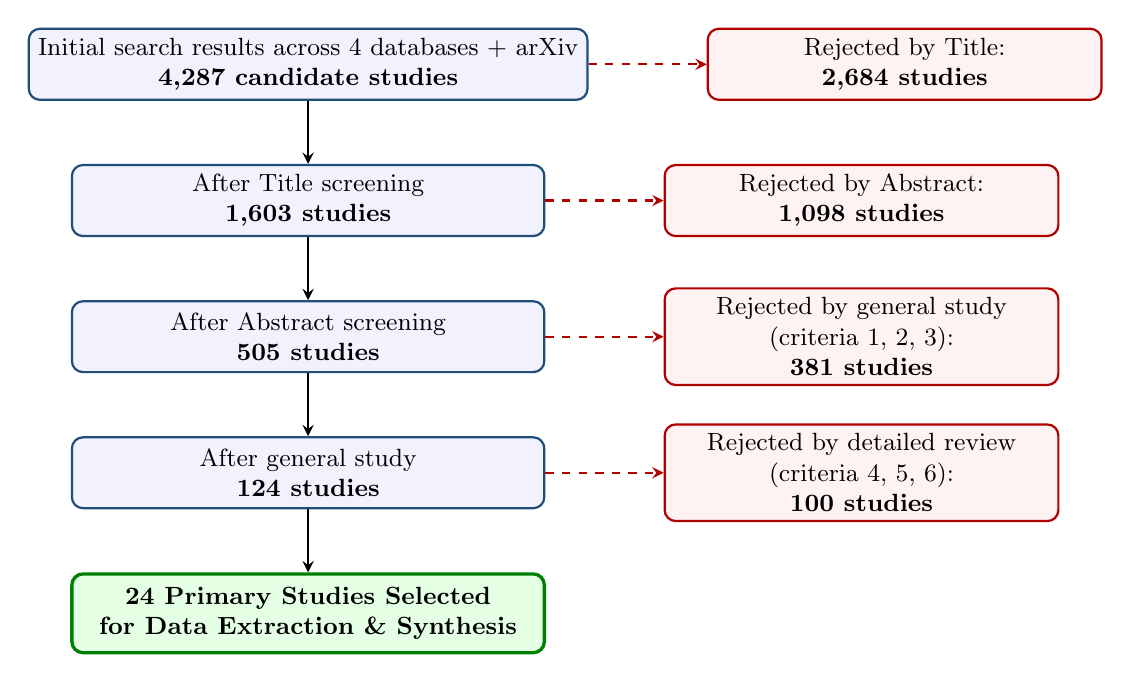
\begin{tikzpicture}[
    node distance=0.8cm and 1.5cm,
    box/.style={
        rectangle,
        rounded corners,
        draw=headerblue,
        thick,
        minimum width=6cm,
        minimum height=0.9cm,
        align=center,
        fill=blue!5,
        font=\small
    },
    rejectbox/.style={
        rectangle,
        rounded corners,
        draw=red!70!black,
        thick,
        minimum width=5cm,
        minimum height=0.8cm,
        align=center,
        fill=red!5,
        font=\small
    },
    finalbox/.style={
        rectangle,
        rounded corners,
        draw=green!50!black,
        very thick,
        minimum width=6cm,
        minimum height=1.0cm,
        align=center,
        fill=green!10,
        font=\small\bfseries
    },
    arrow/.style={-stealth, thick},
    rejectarrow/.style={-stealth, thick, red!70!black, dashed}
]

\node[box] (s1) {Initial search results across 4 databases + arXiv \\ \textbf{4{,}287 candidate studies}};
\node[rejectbox, right=of s1] (r1) {Rejected by Title: \\ \textbf{2{,}684 studies}};
\node[box, below=of s1] (s2) {After Title screening \\ \textbf{1{,}603 studies}};
\node[rejectbox, right=of s2] (r2) {Rejected by Abstract: \\ \textbf{1{,}098 studies}};
\node[box, below=of s2] (s3) {After Abstract screening \\ \textbf{505 studies}};
\node[rejectbox, right=of s3] (r3) {Rejected by general study \\ (criteria 1, 2, 3): \\ \textbf{381 studies}};
\node[box, below=of s3] (s4) {After general study \\ \textbf{124 studies}};
\node[rejectbox, right=of s4] (r4) {Rejected by detailed review \\ (criteria 4, 5, 6): \\ \textbf{100 studies}};
\node[finalbox, below=of s4] (s5) {\textbf{24 Primary Studies Selected} \\ for Data Extraction \& Synthesis};

\draw[arrow] (s1) -- (s2);
\draw[arrow] (s2) -- (s3);
\draw[arrow] (s3) -- (s4);
\draw[arrow] (s4) -- (s5);
\draw[rejectarrow] (s1) -- (r1);
\draw[rejectarrow] (s2) -- (r2);
\draw[rejectarrow] (s3) -- (r3);
\draw[rejectarrow] (s4) -- (r4);

\end{tikzpicture}
\caption{PRISMA-inspired filtering diagram of the SLR search and selection process.}
\label{fig:prisma}
\end{figure}

The six-step filtering process is summarized as follows:

\begin{enumerate}[leftmargin=*]
\item Specify various search terms in five sources and analyze approximately 4{,}287 search results (after deduplication) as per the inclusion/exclusion criteria.
\item Discard 2{,}684 researches by reading their Title as per selection and rejection criteria.
\item Discard 1{,}098 researches by reading their Abstract as per selection and rejection criteria.
\item Perform general study of 505 researches by reading different relevant sections. On the basis of this general study, discard 381 researches that do not meet criteria 1, 2, or 3.
\item Perform detailed study of 124 researches and discard 100 researches that fail to meet the crucial-effects, results-oriented, or repetition criteria.
\item Select \textbf{24 primary researches} fully compliant with all six pre-defined selection criteria for detailed data extraction and synthesis.
\end{enumerate}

%====================================================================
% SECTION 2.1.6 — QUALITY ASSESSMENT
%====================================================================
\subsection{Quality Assessment}
\label{sec:quality_assessment}

A quality criterion has been developed to understand the important outcomes of selected researches and to define the credibility of each selected research and its decisive findings:

\begin{enumerate}[leftmargin=*]
\item The data appraisal of the research is based on concrete facts and theoretical perspective without any vague statements.
\item The validation of research has been performed through proper validation methods (e.g., benchmark evaluation, human assessment, ablation studies).
\item The research provides information about the tools, models, and datasets used in its work, enabling reproducibility.
\item The objective is to include the most recent researches as much as possible. Therefore, 83\% of the selected researches are from 2023 to 2025, and overall 100\% are included from 2021 to 2025, as shown in Figure~\ref{fig:year_distribution}.
\item Originality of the research is another important factor. Therefore, only researches published in at least one of the four renowned scientific databases (IEEE, Springer, Elsevier, ACM) or highly-cited preprints accepted at top venues are included.
\end{enumerate}

\begin{figure}[H]
\centering
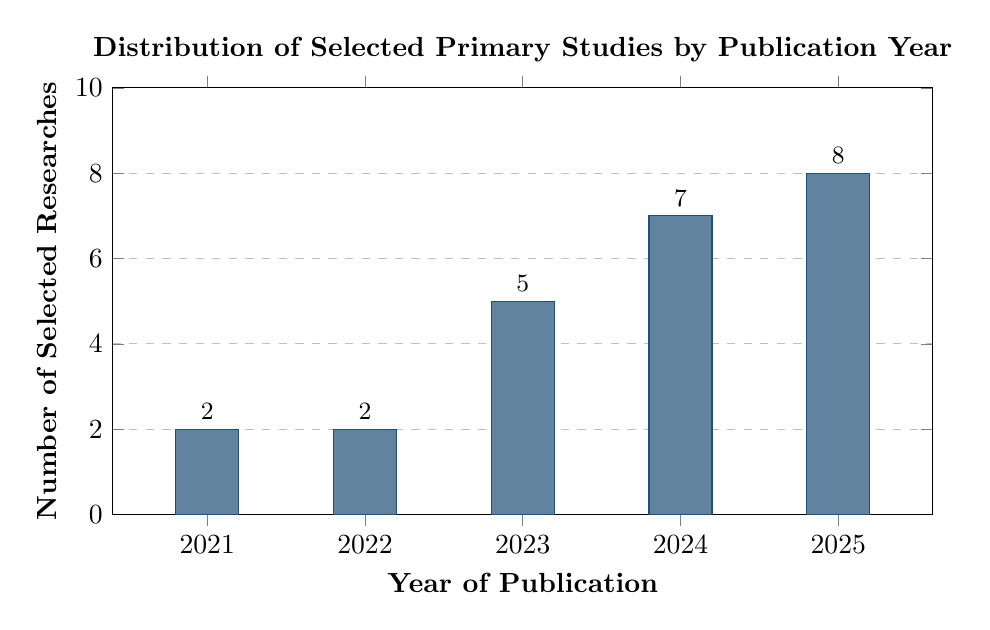
\begin{tikzpicture}
\begin{axis}[
    ybar,
    width=12cm,
    height=7cm,
    bar width=0.8cm,
    ymin=0,
    ymax=10,
    ylabel={\textbf{Number of Selected Researches}},
    xlabel={\textbf{Year of Publication}},
    symbolic x coords={2021,2022,2023,2024,2025},
    xtick=data,
    nodes near coords,
    nodes near coords style={font=\small\bfseries},
    ymajorgrids=true,
    grid style=dashed,
    title={\textbf{Distribution of Selected Primary Studies by Publication Year}},
    enlarge x limits=0.15
]
\addplot[fill=headerblue!70,draw=headerblue] coordinates {
    (2021,2) (2022,2) (2023,5) (2024,7) (2025,8)
};
\end{axis}
\end{tikzpicture}
\caption{Quality assessment showing the temporal distribution of selected primary studies.}
\label{fig:year_distribution}
\end{figure}

%====================================================================
% SECTION 2.1.7 — DATA EXTRACTION AND SYNTHESIS
%====================================================================
\subsection{Data Extraction and Synthesis}
\label{sec:data_extraction}

Data extraction and synthesis, as shown in Table~\ref{tab:data_extraction}, were performed for each selected research in order to obtain the answers to the research questions. The ten attributes cover both bibliographic extraction and analytical synthesis.

\begin{table}[H]
\centering
\caption{Data extraction and synthesis attributes for each selected research.}
\label{tab:data_extraction}
\small
\begin{tabular}{@{}cp{4cm}p{9cm}@{}}
\toprule
\textbf{\#} & \textbf{Attribute} & \textbf{Description} \\
\midrule
\multicolumn{3}{l}{\textit{Extraction of Data}} \\
\midrule
1 & Bibliographic information & Title, author(s), publication year, publisher details, and type (journal/conference/preprint) \\
2 & Overview & The basic proposal and objective of the selected research \\
3 & Results & Quantitative and qualitative results obtained \\
4 & Data collection & Nature of data used (synthetic, benchmark, real-world repositories) \\
5 & Assumptions & Assumptions (if any) required to validate results \\
6 & Validation & Validation method used (benchmark, case study, human evaluation, ablation) \\
\midrule
\multicolumn{3}{l}{\textit{Synthesis of Data}} \\
\midrule
7 & Classification & Relevance to one of the six predefined categories \\
8 & Techniques utilized & Prompting, fine-tuning, RL, multi-agent, retrieval, static analysis, etc. \\
9 & Repair/Optimization mechanism & Self-critique, CDCL backtracking, genetic algorithms, RCI, etc. \\
10 & Tools/Benchmarks identification & Tools, frameworks, and benchmarks used \\
\bottomrule
\end{tabular}
\end{table}

%====================================================================
% SECTION 2.2 — RESULTS
%====================================================================
\section{Results}
\label{sec:results}

Twenty-four primary studies were identified and classified across the six categories. The results are presented through structured synthesis tables, following the methodological guidelines that favor quantitative classification over paragraph-based summaries.

\subsection{Classification of Selected Researches}
\label{sec:classification}

Table~\ref{tab:classification} summarizes the classification of the 24 selected researches into the six predefined categories.

\begin{table}[H]
\centering
\caption{Classification of selected researches across the six predefined categories.}
\label{tab:classification}
\small
\begin{tabular}{@{}clcp{7.5cm}@{}}
\toprule
\textbf{\#} & \textbf{Category} & \textbf{Count} & \textbf{Research Identification} \\
\midrule
1 & General & 5 & Bai et al.~\cite{bai2025agent}, Zhang et al.~\cite{zhang2025anncoder} (AnnCoder), Ding et al.~\cite{ding2025codingcare} (CodingCare), Dou et al.~\cite{dou2026}, Zhang et al.~\cite{zhang2025abfcg} (ABFCG) \\
\midrule
2 & Code Generation & 6 & Li et al.~\cite{li2025scot} (SCoT), Jiang et al.~\cite{jiang2024selfplan} (Self-Planning), Wei et al.~\cite{wei2022cot} (CoT), Chen et al.~\cite{chen2021humaneval} (HumanEval), Austin et al.~\cite{austin2021mbpp} (MBPP), Hendrycks et al.~\cite{hendrycks2021apps} (APPS) \\
\midrule
3 & Bug Detection \& Classification & 1 & Dou et al.~\cite{dou2026}* \\
\midrule
4 & Code Repair & 6 & Xia et al.~\cite{xia2023apr}, Chen et al.~\cite{chen2023selfdebug} (Self-Debug), Wang et al.~\cite{wang2024intervenor} (Intervenor), Frenkel et al.~\cite{frenkel2025apr}, Zhang et al.~\cite{zhang2024copilot} (Copilot-in-the-Loop), Liu et al.~\cite{liu2025llm4tdg} (LLM4TDG) \\
\midrule
5 & Code Optimization & 3 & Zhao et al.~\cite{zhao2025semopt} (SemOpt), Jonnala et al.~\cite{jonnala2025} (Efficiency), Lyu et al.~\cite{lyu2025toppass} (Top Pass) \\
\midrule
6 & Security & 3 & Bruni et al.~\cite{bruni2025}, Nazzal et al.~\cite{nazzal2024promsec} (PromSec), Ding et al.~\cite{ding2025codingcare}* \\
\midrule
\multicolumn{2}{r}{\textbf{Total distinct studies:}} & \textbf{24} & \\
\bottomrule
\end{tabular}
\begin{flushleft}
\footnotesize * indicates studies appearing in multiple categories due to their multi-faceted contributions.
\end{flushleft}
\end{table}

\subsection{Prompting and Reasoning Techniques Utilization}
\label{sec:prompting_results}

Table~\ref{tab:prompting_techniques} summarizes the utilization of prompting and reasoning techniques across the selected researches.

\begin{table}[H]
\centering
\caption{Prompting and reasoning techniques utilized in selected researches.}
\label{tab:prompting_techniques}
\small
\begin{tabular}{@{}clcp{7cm}@{}}
\toprule
\textbf{\#} & \textbf{Technique} & \textbf{Count} & \textbf{Relevant Researches} \\
\midrule
1 & Zero-shot prompting & 4 & \cite{chen2021humaneval,austin2021mbpp,hendrycks2021apps,xia2023apr} \\
2 & Few-shot prompting & 6 & \cite{austin2021mbpp,li2025scot,jiang2024selfplan,wei2022cot,chen2023selfdebug,wang2024intervenor} \\
3 & Chain-of-Thought (CoT) & 9 & \cite{wei2022cot,li2025scot,jonnala2025,bai2025agent,bruni2025,ding2025codingcare,dou2026,wang2024intervenor,chen2023selfdebug} \\
4 & Structured Chain-of-Thought (SCoT) & 2 & \cite{li2025scot,zhang2025anncoder} \\
5 & Self-Planning & 3 & \cite{jiang2024selfplan,zhang2025anncoder,bai2025agent} \\
6 & Recursive Criticism \& Improvement (RCI) & 3 & \cite{bruni2025,ding2025codingcare,dou2026} \\
7 & Role-based prompting (multi-agent) & 5 & \cite{bai2025agent,zhang2025anncoder,ding2025codingcare,wang2024intervenor,frenkel2025apr} \\
8 & Self-critique prompting & 4 & \cite{dou2026,chen2023selfdebug,wang2024intervenor,zhang2024copilot} \\
\bottomrule
\end{tabular}
\end{table}

From Table~\ref{tab:prompting_techniques}, Chain-of-Thought (CoT) emerges as the most frequently utilized technique, appearing in 9 of 24 (37.5\%) selected studies. Its structured variant (SCoT) and self-planning extensions collectively account for another 5 studies (20.8\%), indicating a strong trend toward structured intermediate reasoning in modern LLM code generation research.

\subsection{Bug Repair Approaches Utilization}
\label{sec:repair_results}

Table~\ref{tab:repair_approaches} summarizes the bug detection and repair approaches utilized across the selected researches.

\begin{table}[H]
\centering
\caption{Bug detection and repair approaches in selected researches.}
\label{tab:repair_approaches}
\small
\begin{tabular}{@{}clcp{7cm}@{}}
\toprule
\textbf{\#} & \textbf{Approach} & \textbf{Count} & \textbf{Relevant Researches} \\
\midrule
1 & Self-critique with compiler feedback & 6 & \cite{dou2026,chen2023selfdebug,wang2024intervenor,zhang2024copilot,bai2025agent,ding2025codingcare} \\
2 & Constraint-based reasoning (CDG/CDCL) & 1 & \cite{liu2025llm4tdg} \\
3 & Multi-agent collaborative review & 4 & \cite{bai2025agent,zhang2025anncoder,ding2025codingcare,frenkel2025apr} \\
4 & Static analysis integration (CodeQL/Semgrep/Bandit) & 4 & \cite{bruni2025,ding2025codingcare,nazzal2024promsec,zhao2025semopt} \\
5 & Evolutionary optimization (SA + GA) & 1 & \cite{zhang2025anncoder} \\
6 & Ranking-based candidate selection & 1 & \cite{lyu2025toppass} \\
7 & Formal verification-based repair & 1 & \cite{frenkel2025apr} \\
8 & Bug taxonomy-driven repair & 2 & \cite{dou2026,zhang2024copilot} \\
\bottomrule
\end{tabular}
\end{table}

Among the constraint‑based approaches, \cite{liu2025llm4tdg} stands out by combining a constraint dependency graph with conflict‑driven clause learning (CDCL) to iteratively repair syntactic and semantic errors in test drivers. Their framework achieves a 47.62\% constraint understanding gain and raises the average \texttt{pass@k} of nine LLMs by 10.41\% (up to 18.66\% for CodeQwen‑chat) on HUMANEVAL and HUMANEVAL+. It further demonstrates effectiveness on real‑world security testing tasks, detecting malicious behavior in compromised PyPI dependency libraries by generating correct, executable test cases.

\subsection{Benchmarks and Evaluation Datasets}
\label{sec:benchmarks_results}

Table~\ref{tab:benchmarks} summarizes the benchmarks used for evaluation across the selected researches.

\begin{table}[H]
\centering
\caption{Benchmarks and evaluation datasets utilized in selected researches.}
\label{tab:benchmarks}
\small
\begin{tabular}{@{}clcp{6cm}@{}}
\toprule
\textbf{\#} & \textbf{Benchmark} & \textbf{Count} & \textbf{Key Characteristics} \\
\midrule
1 & HumanEval/HumanEval+ & 14 & 164 Python problems, pass@k metric \\
2 & MBPP/MBPP+ & 11 & 974 crowd-sourced entry-level problems \\
3 & APPS/APPS+ & 6 & 10{,}000 competitive programming problems \\
4 & EffiBench & 1 & 243 greedy-algorithm efficiency problems \\
5 & LLMSecEval & 2 & 150 CWE-mapped security prompts \\
6 & SecurityEval & 1 & 130 security-focused prompts \\
7 & CodeContests & 1 & 13{,}000+ competitive problems \\
8 & SWE-bench (GitHub issues) & 1 & Real-world repository bugs \\
9 & RWPB (Dou et al.) & 1 & 140 real-world 2024 GitHub tasks \\
9.5 & pypi\_malregistry & 1 & 5 real-world malicious Python packages; Security (dynamic testing) \\
10 & Real-world web projects (5 types) & 1 & E-commerce, forum, blog, news, admin \\
\bottomrule
\end{tabular}
\end{table}

\subsection{Preliminary Tools and Frameworks Identification}
\label{sec:tools_prelim}

Table~\ref{tab:tools_prelim} presents the preliminary identification of tools and frameworks utilized in the selected researches, grouped by their primary LLM-based code generation activity.

\begin{table}[H]
\centering
\caption{Preliminary tools and frameworks identified in selected researches.}
\label{tab:tools_prelim}
\small
\begin{tabular}{@{}clp{8cm}@{}}
\toprule
\textbf{\#} & \textbf{Tool/Framework} & \textbf{Relevant Researches} \\
\midrule
\multicolumn{3}{l}{\textit{Generation Frameworks (6)}} \\
\midrule
1 & ChatDev~\cite{qian2023chatdev} & \cite{bai2025agent,zhang2025anncoder} \\
2 & MetaGPT~\cite{hong2023metagpt} & \cite{zhang2025anncoder,ding2025codingcare} \\
3 & AutoGen~\cite{wu2023autogen} & \cite{bai2025agent,frenkel2025apr} \\
4 & Self-Planning~\cite{jiang2024selfplan} & \cite{jiang2024selfplan} \\
5 & SCoT~\cite{li2025scot} & \cite{li2025scot} \\
6 & ABFCG~\cite{zhang2025abfcg} & \cite{zhang2025abfcg} \\
\midrule
\multicolumn{3}{l}{\textit{Bug Repair \& Test Generation Tools (5)}} \\
\midrule
7 & LLM4TDG~\cite{liu2025llm4tdg} & \cite{liu2025llm4tdg} \\
8 & Self-Debug~\cite{chen2023selfdebug} & \cite{chen2023selfdebug,dou2026} \\
9 & Intervenor~\cite{wang2024intervenor} & \cite{wang2024intervenor,dou2026} \\
10 & AnnCoder~\cite{zhang2025anncoder} & \cite{zhang2025anncoder} \\
11 & Copilot-in-the-Loop~\cite{zhang2024copilot} & \cite{zhang2024copilot} \\
\midrule
\multicolumn{3}{l}{\textit{Static Analysis Tools (3)}} \\
\midrule
12 & CodeQL & \cite{bruni2025,ding2025codingcare,bai2025agent} \\
13 & Semgrep & \cite{bruni2025,zhao2025semopt,ding2025codingcare} \\
14 & Bandit & \cite{ding2025codingcare} \\
\midrule
\multicolumn{3}{l}{\textit{Security \& Optimization Tools (4)}} \\
\midrule
15 & PromSec~\cite{nazzal2024promsec} & \cite{nazzal2024promsec} \\
16 & CodingCare~\cite{ding2025codingcare} & \cite{ding2025codingcare} \\
17 & SemOpt~\cite{zhao2025semopt} & \cite{zhao2025semopt} \\
18 & Top Pass~\cite{lyu2025toppass} & \cite{lyu2025toppass} \\
\bottomrule
\end{tabular}
\end{table}

%====================================================================
% SECTION 2.3 — COMPARISON
%====================================================================
\section{Comparison}
\label{sec:comparison}

A comprehensive comparative evaluation of the identified tools and frameworks is performed using both general and activity-specific characteristics. The general characteristics include license type, customizability, and supported models, while activity-specific characteristics vary based on the tool's primary function (generation, repair, optimization, or security).

\subsection{Tools Characteristics Defined}
\label{sec:char_defined}

\subsubsection*{2.3.1.1 General Characteristics}

\begin{itemize}[leftmargin=*]
\item \textbf{License Type:} Open-source (MIT, Apache-2.0, GPL, MPL) or Proprietary.
\item \textbf{Customizability:} Full (source code modifiable), Partial (configuration/extension supported), No (closed).
\item \textbf{Supported LLMs:} Models the tool is compatible with (e.g., GPT-4, Claude-3, DeepSeek, Llama-3).
\end{itemize}

\subsubsection*{2.3.1.2 Activity-Specific Characteristics}

\begin{itemize}[leftmargin=*]
\item \textbf{Generation tools:} Supported prompting strategies (CoT/SCoT/Self-Planning), multi-agent support.
\item \textbf{Repair tools:} Feedback source (compiler/unit tests/static analysis), iteration support.
\item \textbf{Optimization tools:} Optimization dimension (correctness/efficiency/readability), algorithm type.
\item \textbf{Security tools:} CWE coverage, detection method (static/dynamic/hybrid).
\end{itemize}

\subsection{Comparison of Code Generation Frameworks}

\begin{table}[H]
\centering
\caption{Comparison of code generation frameworks used in LLM-based code generation.}
\label{tab:cmp_generation}
\scriptsize
\begin{tabular}{@{}lcccccc@{}}
\toprule
\multirow{2}{*}{\textbf{Tool Name}} & \multicolumn{3}{c}{\textbf{General Characteristics}} & \multicolumn{3}{c}{\textbf{Activity-Specific Characteristics}} \\
\cmidrule(lr){2-4} \cmidrule(lr){5-7}
 & \textbf{License} & \textbf{Customizability} & \textbf{Supported LLMs} & \textbf{CoT Support} & \textbf{Multi-Agent} & \textbf{Planning} \\
\midrule
ChatDev~\cite{qian2023chatdev} & Apache-2.0 & Full & GPT-3.5/4 & Yes & Yes & Yes \\
MetaGPT~\cite{hong2023metagpt} & MIT & Full & GPT-3.5/4, Claude & Yes & Yes & Yes (SOP-based) \\
AutoGen~\cite{wu2023autogen} & MIT & Full & Multi-LLM & Yes & Yes & Flexible \\
Self-Planning~\cite{jiang2024selfplan} & N/A (prompt method) & Full & Any LLM & Yes & No & Yes \\
SCoT~\cite{li2025scot} & N/A (prompt method) & Full & Any LLM & Structured & No & Implicit \\
ABFCG~\cite{zhang2025abfcg} & N/A & Partial & Custom (RetNet) & No & No & No (KG-based) \\
Bai et al.~\cite{bai2025agent} & Proprietary & Partial & GPT-3.5/4 & Yes & Yes (BART agent) & Yes \\
\bottomrule
\end{tabular}
\end{table}

\subsection{Comparison of Bug Detection and Repair Tools}

\begin{table}[H]
\centering
\caption{Comparison of bug detection and automated repair tools.}
\label{tab:cmp_repair}
\scriptsize
\begin{tabular}{@{}lcccccc@{}}
\toprule
\multirow{2}{*}{\textbf{Tool Name}} & \multicolumn{3}{c}{\textbf{General Characteristics}} & \multicolumn{3}{c}{\textbf{Activity-Specific Characteristics}} \\
\cmidrule(lr){2-4} \cmidrule(lr){5-7}
 & \textbf{License} & \textbf{Custom.} & \textbf{Supported LLMs} & \textbf{Feedback} & \textbf{Iterative} & \textbf{Taxonomy} \\
\midrule
LLM4TDG~\cite{liu2025llm4tdg} & Open-source & Full & 9 LLMs & Runtime + CDG & Yes (CDCL) & No (constraint‑driven) \\
Self-Debug~\cite{chen2023selfdebug} & N/A & Full & Any LLM & Compiler & Yes & No \\
Intervenor~\cite{wang2024intervenor} & Open-source & Full & GPT-4 + student & Compiler + CoT & Yes & No \\
Dou et al.~\cite{dou2026} & Open-source & Full & 9 LLMs & Compiler + Taxonomy & Yes (2-iter) & 3 primary / 10 secondary \\
Xia et al.~\cite{xia2023apr} & Research & Full & 9 LLMs (Codex etc.) & Unit tests & Optional & No \\
Frenkel et al.~\cite{frenkel2025apr} & Academic & Partial & N/A (SMT-based) & SMT solver & Yes (AGR) & Formal \\
Copilot-in-the-Loop~\cite{zhang2024copilot} & Proprietary & No & Copilot Chat & Smell name & Yes & Pysmell-based \\
AnnCoder~\cite{zhang2025anncoder} & Research & Partial & GPT-3.5/4-Turbo & Test + SA/GA & Yes & Evolutionary \\
\bottomrule
\end{tabular}
\end{table}

\subsection{Comparison of Code Optimization Tools}

\begin{table}[H]
\centering
\caption{Comparison of code optimization tools and techniques.}
\label{tab:cmp_optimization}
\scriptsize
\begin{tabular}{@{}lcccccc@{}}
\toprule
\multirow{2}{*}{\textbf{Tool Name}} & \multicolumn{3}{c}{\textbf{General Characteristics}} & \multicolumn{3}{c}{\textbf{Activity-Specific Characteristics}} \\
\cmidrule(lr){2-4} \cmidrule(lr){5-7}
 & \textbf{License} & \textbf{Custom.} & \textbf{Supported LLMs} & \textbf{Dimension} & \textbf{Algorithm} & \textbf{Languages} \\
\midrule
SemOpt~\cite{zhao2025semopt} & Open-source & Full & DeepSeek-V3, GPT-4.1, Gemini-2.5 & Efficiency & Rule-based (Semgrep) & C/C++ \\
Jonnala et al.~\cite{jonnala2025} & N/A & Full & GPT-3.5/4/4o-Mini & Time + Memory & CoT + Fine-tuning & Python \\
Top Pass~\cite{lyu2025toppass} & Open-source & Full & ChatGPT, DeepSeek-Coder & Ranking & pass@k loss & Multi \\
AnnCoder~\cite{zhang2025anncoder} & Research & Partial & GPT-3.5/4-Turbo & Multi-dim. & SA + GA & Python \\
\bottomrule
\end{tabular}
\end{table}

\subsection{Comparison of Security Tools}

\begin{table}[H]
\centering
\caption{Comparison of security-focused tools in LLM code generation.}
\label{tab:cmp_security}
\scriptsize
\begin{tabular}{@{}lcccccc@{}}
\toprule
\multirow{2}{*}{\textbf{Tool Name}} & \multicolumn{3}{c}{\textbf{General Characteristics}} & \multicolumn{3}{c}{\textbf{Activity-Specific Characteristics}} \\
\cmidrule(lr){2-4} \cmidrule(lr){5-7}
 & \textbf{License} & \textbf{Custom.} & \textbf{Supported LLMs} & \textbf{CWE Coverage} & \textbf{Detection} & \textbf{Method} \\
\midrule
PromSec~\cite{nazzal2024promsec} & Research & Full & GPT-3.5/4 & High & gGAN + Prompt-loop & Hybrid \\
CodingCare~\cite{ding2025codingcare} & Research & Full & DeepSeek, Mistral, CodeLlama (7B) & $\geq$50\% reduction & CodeQL + Bandit & Static \\
Bruni et al.~\cite{bruni2025} & N/A (evaluation) & Partial & GPT-3.5/4o-Mini/4o & 18+ CWEs & Semgrep + CodeQL & Static \\
\bottomrule
\end{tabular}
\end{table}

\subsection{Comparison of Benchmarks}

\begin{table}[H]
\centering
\caption{Comparison of benchmarks used in LLM code generation research.}
\label{tab:cmp_benchmarks}
\scriptsize
\begin{tabular}{@{}lccccc@{}}
\toprule
\textbf{Benchmark} & \textbf{Size} & \textbf{Language} & \textbf{Source} & \textbf{Focus} & \textbf{Leakage Risk} \\
\midrule
HumanEval~\cite{chen2021humaneval} & 164 & Python & Hand-crafted & Correctness & High (pre-trained exposure) \\
HumanEval+~\cite{chen2021humaneval} & 164 & Python & Augmented tests & Correctness (rigorous) & High \\
MBPP~\cite{austin2021mbpp} & 974 & Python & Crowd-sourced & Entry-level correctness & Moderate \\
MBPP+~\cite{austin2021mbpp} & 399 & Python & Augmented tests & Correctness (rigorous) & Moderate \\
APPS~\cite{hendrycks2021apps} & 10{,}000 & Python & Codeforces/Kattis & Competitive difficulty & Moderate \\
APPS+~\cite{dou2026} & 600 & Python & Curated APPS & Correctness & Low \\
EffiBench~\cite{jonnala2025} & 1{,}000+ & Python & LeetCode greedy & Efficiency & Moderate \\
LLMSecEval~\cite{bruni2025} & 150 & Python/C & CWE-mapped & Security & Low \\
RWPB~\cite{dou2026} & 140 & Python & GitHub 2024 & Real-world correctness & Very Low \\
SWE-bench & Variable & Python & GitHub issues & Real-world repair & Low \\
\bottomrule
\end{tabular}
\end{table}

%====================================================================
% SECTION 2.4 — ANSWERS TO RESEARCH QUESTIONS
%====================================================================
\section{Answers to Research Questions}
\label{sec:answers}

\subsection*{RQ1: What important researches have been reported from 2021 to 2025?}

\textbf{Answer:} Twenty-four important researches published from 2021 to 2025 have been identified as per the selection and rejection criteria (Section~\ref{sec:inclusion_criteria}). These researches are classified into six corresponding categories. The details are as follows:
\begin{itemize}[leftmargin=*]
\item \textbf{Five researches} have been identified in the \textit{General} category, covering multi-aspect LLM code generation (Bai et al., AnnCoder, CodingCare, Dou et al., ABFCG).
\item \textbf{Six researches} have been identified in the \textit{Code Generation} category, with three being foundational benchmark papers (HumanEval, MBPP, APPS) and three being technique-focused works (SCoT, Self-Planning, CoT).
\item \textbf{One research} has been identified in the \textit{Bug Detection \& Classification} category (Dou et al.).
\item \textbf{Six researches} have been identified in the \textit{Code Repair} category (Xia et al., Self-Debug, Intervenor, Frenkel et al., Copilot-in-the-Loop, LLM4TDG).
\item \textbf{Three researches} have been identified in the \textit{Code Optimization} category (SemOpt, Jonnala et al., Top Pass).
\item \textbf{Three researches} have been identified in the \textit{Security} category (Bruni et al., PromSec, CodingCare).
\end{itemize}
The overview, publication year, validation method, and description of each selected technique are summarized in Table~\ref{tab:classification}.

\subsection*{RQ2: Which prompting techniques are more frequently utilized?}

\textbf{Answer:} As analyzed in Table~\ref{tab:prompting_techniques}, Chain-of-Thought (CoT) is the most frequently utilized technique, appearing in 9 of 24 studies (37.5\%). This is followed by few-shot prompting (6 studies, 25.0\%), role-based multi-agent prompting (5 studies, 20.8\%), and self-critique prompting (4 studies, 16.7\%). Structured variants such as SCoT and Self-Planning collectively account for 5 studies (20.8\%). RCI (Recursive Criticism and Improvement) is used in 3 studies (12.5\%). The clear trend is that \textit{structured intermediate reasoning} dominates contemporary LLM code generation research, with nearly 79\% of studies employing some form of explicit reasoning scaffolding.

\subsection*{RQ3: Which bug repair approaches are more frequently utilized?}

\textbf{Answer:} As shown in Table~\ref{tab:repair_approaches}, self-critique with compiler feedback is the most dominant repair approach (6 studies, 25.0\%), followed by multi-agent collaborative review (4 studies, 16.7\%), and static analysis integration (4 studies, 16.7\%). Bug-taxonomy-driven repair, a recent development pioneered by Dou et al., is employed in 2 studies. Constraint-based reasoning (CDG/CDCL), evolutionary optimization (SA + GA), ranking-based selection, and formal verification are each represented by a single study, indicating that these represent specialized but potentially underexplored directions. The convergence on self-critique with compiler feedback suggests it has emerged as a de facto standard for LLM-based repair.

\subsection*{RQ4: What are the significant tools, frameworks, and benchmarks?}

\textbf{Answer:} On the basis of the SLR, 18 tools/frameworks and 10 benchmarks have been identified to support LLM-based code generation across the five activity dimensions. After the comparative evaluation in Section~\ref{sec:comparison}, the following key tools are recommended by activity:
\begin{itemize}[leftmargin=*]
\item \textbf{Seven generation frameworks} are presented to support prompting, planning, and multi-agent orchestration (ChatDev, MetaGPT, AutoGen, Self-Planning, SCoT, ABFCG, Bai et al.).
\item \textbf{Eight bug detection and repair tools} are presented (LLM4TDG, Self-Debug, Intervenor, Dou et al., Xia et al., Frenkel et al., Copilot-in-the-Loop, AnnCoder). Among these, LLM4TDG notably achieves the highest \texttt{pass@k} improvement (18.66\% on CodeQwen‑chat) and validates its approach on real malicious packages, bridging the gap between benchmarks and security testing.
\item \textbf{Four code optimization tools} are presented (SemOpt, Jonnala et al., Top Pass, AnnCoder).
\item \textbf{Three security tools} are presented (PromSec, CodingCare, Bruni et al.).
\item \textbf{Three static analysis integration tools} are consistently used across security-focused works (CodeQL, Semgrep, Bandit).
\item \textbf{Ten benchmarks} span correctness (HumanEval, MBPP, APPS and their augmented variants), efficiency (EffiBench), security (LLMSecEval, SecurityEval), and real-world evaluation (RWPB, SWE-bench).
\end{itemize}

%====================================================================
% SECTION 2.5 — DISCUSSION AND LIMITATIONS
%====================================================================
\section{Discussion and Limitations}
\label{sec:discussion}

\subsection{Discussion on Code Generation Techniques}

It is analyzed that prompting and reasoning scaffolds are the core enablers of LLM-based code generation. The evolution from zero-shot prompting through CoT to SCoT and Self-Planning reveals a systematic trend: \textit{the more structured the intermediate representation, the better the downstream code quality}. Structured variants such as SCoT achieve up to 13.79\% improvement over vanilla CoT on HumanEval \cite{li2025scot}, validating this hypothesis empirically. Moreover, reasoning-specialized models (e.g., DeepSeek-R1) that internalize structured reasoning achieve even higher gains (up to 77.9\% on RWPB~\cite{dou2026}), suggesting that the trajectory of future research lies in combining explicit scaffolding with reasoning-enhanced model architectures.

\subsection{Discussion on Bug Detection and Repair}

Bug taxonomy construction (e.g., Dou et al.'s 3-primary/10-secondary classification) provides essential analytical infrastructure for systematic repair. Self-critique with compiler feedback, often combined with bug-taxonomy-driven prompts, achieves a 29.2\% repair success rate after two iterations on state-of-the-art models. However, functional bugs, which account for the highest proportion of errors, remain the hardest to repair, with transformation rates (functional $\to$ correct) lagging behind syntax and runtime bug repair. This indicates that functional correctness demands deeper semantic understanding that current LLMs, even with iterative feedback, do not fully possess.

In contrast, LLM4TDG~\cite{liu2025llm4tdg} shows that constraint‑driven iterative repair not only improves benchmark scores but also uncovers malicious code in real‑world dependency libraries, hinting at its potential for integrated security and correctness validation.

\subsection{Discussion on Optimization and Security}

Optimization research reveals that efficiency gains are hardware- and model-dependent: CoT prompting improves efficiency for smaller models but can be neutral or counterproductive for larger ones \cite{jonnala2025}. High-CPU hardware configurations consistently outperform high-memory configurations for LLM-generated code. On the security front, the finding that the security-focused prefix \textit{``You are a developer who is very security-aware''} reduces vulnerable code by up to 56\% on GPT-4o \cite{bruni2025} demonstrates the remarkable power of simple prompt engineering. However, this effect does not generalize to weaker models (GPT-3.5), where the same prefix can increase vulnerabilities by 31\%, underscoring the importance of model-aware prompt design.

\subsection{Discussion on LLM-Based Tools Selection}

The selection of appropriate LLM-based code generation tools is always challenging due to the wide-ranging characteristics of code generation tasks. Moreover, seamless integration of different tools within a single pipeline is another problem. From this research, it has been analyzed that multi-agent frameworks (ChatDev, MetaGPT, AutoGen) are playing the leading role by providing flexible orchestration for multiple activities. Various specialized tools are built on top of these frameworks (e.g., AnnCoder, Bai et al.'s framework, CodingCare). Further, these frameworks are highly customizable and can be altered according to diverse LLM-based code generation requirements.

\subsection{Limitations of Research}

Although we have completely followed the guidelines of SLR and strictly observed the developed review protocol, there are still certain limitations:

\begin{itemize}[leftmargin=*]
\item We have used appropriate search terms and thoroughly scanned the search results. However, few search terms returned thousands of results that cannot be scanned exhaustively. Furthermore, we have rejected a number of researches based on their titles, and there is a possibility that the contents of such researches are not properly reflected in the titles. Consequently, we do not claim the exhaustiveness of our research.

\item We have used five sources (four renowned scientific databases plus arXiv). These sources provide a large amount of journal and conference publications. However, some relevant research work may be provided by other sources (e.g., OpenReview, semantic archives). Therefore, there is a fair chance that we have missed some relevant researches. However, we believe that the ultimate findings of this SLR are not affected significantly because the selected sources provide high-quality recent research literature.

\item The field of LLM-based code generation is evolving extraordinarily rapidly, with new techniques emerging on a monthly basis. Our cutoff of 2025 may therefore exclude very recent developments. Future SLR updates will be required to maintain currency.
\end{itemize}

%====================================================================
% SECTION 2.6 — RESEARCH GAP AND MACI JUSTIFICATION
%====================================================================
\section{Research Gap and MACI Justification}
\label{sec:research_gap}

The synthesis of 24 primary studies reveals several critical research gaps that collectively motivate the development of Multi-Agent Collaborative Intelligence (MACI) frameworks for code generation.

\subsection{Identified Research Gaps}

\textbf{Gap 1: Fragmented Treatment of Multi-Dimensional Quality.} Contemporary research predominantly targets a single quality dimension (correctness, efficiency, or security) in isolation. Only 5 of 24 studies (20.8\%) address multiple dimensions simultaneously (General category). No single framework integrates correctness-aware generation (SCoT/Self-Planning), efficiency optimization (SemOpt), security assurance (CodingCare/PromSec), and iterative repair (Self-Debug/Intervenor) into a unified pipeline.

\textbf{Gap 2: Limited Taxonomy-Aware Multi-Agent Repair.} While Dou et al.~\cite{dou2026} introduced a rigorous bug taxonomy and Bai et al.~\cite{bai2025agent} introduced agent-based review, no existing work combines \textit{bug-taxonomy-driven reasoning} with \textit{multi-agent role specialization}. The current self-critique paradigm operates within a single-agent loop, missing the benefits of role-based division of labor demonstrated by ChatDev, MetaGPT, and AutoGen.

\textbf{Gap 3: Weak Integration of Formal and Probabilistic Methods.} Formal verification approaches (LLM4TDG's CDCL, Frenkel et al.'s SMT-based repair) and probabilistic LLM-based methods operate in silos. A hybrid framework that uses formal constraint reasoning to \textit{guide} LLM generation and uses LLM reasoning to \textit{accelerate} formal verification remains largely unexplored.

\textbf{Gap 4: Insufficient Real-World Benchmark Coverage.} Of the 10 identified benchmarks, only RWPB and SWE-bench target real-world scenarios with low data-leakage risk. The field remains heavily dependent on HumanEval/MBPP/APPS, which may not reflect production software engineering complexity and have demonstrable leakage risks \cite{dou2026}.

\textbf{Gap 5: Limited Language and Paradigm Diversity.} The overwhelming majority of reviewed studies (22 of 24, 91.7\%) focus on Python. Compiled languages (Java, C++, Rust), functional languages, and domain-specific languages are severely underrepresented, limiting the generalizability of current findings.

\subsection{MACI as a Unified Response}

A Multi-Agent Collaborative Intelligence (MACI) framework directly addresses Gaps 1--4 by orchestrating specialized agents, each encoding expertise from one research thread, through structured communication and iterative refinement. A proposed MACI architecture would integrate:

\begin{itemize}[leftmargin=*]
\item A \textbf{Planning Agent} employing SCoT/Self-Planning for structured decomposition (Gap 1, generation dimension).
\item A \textbf{Coding Agent} with retrieval-augmented knowledge base (ABFCG-style) for context-aware synthesis (Gap 1).
\item A \textbf{Bug Detection Agent} leveraging Dou et al.'s bug taxonomy for fine-grained error classification (Gaps 1, 2).
\item A \textbf{Repair Agent} combining self-critique, compiler feedback, and CDCL-style constraint reasoning (Gaps 2, 3).
\item A \textbf{Security Agent} integrating CodeQL/Semgrep static analysis and CWE-aware prompt engineering (Gap 1, security dimension).
\item An \textbf{Optimization Agent} applying SemOpt-style rule-based transformations and efficiency-aware ranking (Gap 1, efficiency dimension).
\item An \textbf{Orchestrator} using AutoGen-style conversation patterns to coordinate agent interactions.
\end{itemize}

Such a framework would represent the first unified response to the multi-dimensional quality demands of production software, leveraging the complementary strengths identified across the 24 reviewed studies. The evidence base compiled in this SLR, comprising validated techniques, tools, and benchmarks, provides the foundation upon which a MACI framework can be rigorously designed and evaluated.

%====================================================================
% SECTION 2.7 — SUMMARY
%====================================================================
\section{Conclusions}
\label{sec:summary}

This Systematic Literature Review has rigorously identified, classified, and analyzed 24 primary studies on LLM-based code generation published between 2021 and 2025. Following a structured review protocol encompassing precise research questions, six concrete selection criteria, a multi-stage filtering process yielding 24 primary studies from an initial pool of 4{,}287 candidates, and a comprehensive data extraction framework, the review provides an evidence-based synthesis of contemporary techniques, tools, and benchmarks.

The key findings are fourfold. First, Chain-of-Thought prompting and its structured variants dominate contemporary research, with 79\% of studies employing some form of structured intermediate reasoning. Second, self-critique with compiler feedback has emerged as the de facto standard for automated bug repair, achieving up to 29.2\% repair success rates in two iterations. Third, multi-agent frameworks (ChatDev, MetaGPT, AutoGen) provide the architectural foundation upon which specialized generation, repair, optimization, and security tools are increasingly built. Fourth, significant research gaps remain in the integration of multi-dimensional quality (correctness + efficiency + security), the combination of formal verification with probabilistic LLM reasoning, the availability of leakage-free real-world benchmarks, and the diversity of programming language coverage.

These findings directly motivate the development of Multi-Agent Collaborative Intelligence (MACI) frameworks that unify the complementary strengths identified across the reviewed literature. By orchestrating specialized agents through structured communication and iterative refinement, MACI-style systems promise to deliver code that is simultaneously correct, efficient, secure, and maintainable, thereby narrowing the gap between laboratory benchmarks and real-world deployment requirements.

%====================================================================
% REFERENCES
%====================================================================
\begin{thebibliography}{99}
\footnotesize

\bibitem{dou2026}
S. Dou, H. Jia, S. Wu, H. Zheng, M. Wu et al., ``What is wrong with your code generated by large language models? An extensive study,'' \textit{Science China Information Sciences}, vol. 69, no. 1, p. 112107, 2026.

\bibitem{chen2021humaneval}
M. Chen, J. Tworek, H. Jun, Q. Yuan et al., ``Evaluating large language models trained on code,'' \textit{arXiv preprint arXiv:2107.03374}, 2021.

\bibitem{austin2021mbpp}
J. Austin, A. Odena, M. Nye, M. Bosma et al., ``Program synthesis with large language models,'' \textit{arXiv preprint arXiv:2108.07732}, 2021.

\bibitem{hendrycks2021apps}
D. Hendrycks, S. Basart, S. Kadavath, M. Mazeika et al., ``Measuring coding challenge competence with APPS,'' \textit{arXiv preprint arXiv:2105.09938}, 2021.

\bibitem{wei2022cot}
J. Wei, X. Wang, D. Schuurmans, M. Bosma et al., ``Chain-of-thought prompting elicits reasoning in large language models,'' \textit{Advances in Neural Information Processing Systems (NeurIPS)}, vol. 35, pp. 24824--24837, 2022.

\bibitem{li2025scot}
J. Li, G. Li, Y. Li, and Z. Jin, ``Structured chain-of-thought prompting for code generation,'' \textit{ACM Transactions on Software Engineering and Methodology}, vol. 34, no. 2, Article 37, 2025.

\bibitem{jiang2024selfplan}
X. Jiang, Y. Dong, L. Wang, Z. Fang, Q. Shang, G. Li, Z. Jin, and W. Jiao, ``Self-planning code generation with large language models,'' \textit{ACM Transactions on Software Engineering and Methodology}, vol. 33, pp. 1--30, 2024.

\bibitem{qian2023chatdev}
C. Qian, X. Cong, W. Liu, C. Yang et al., ``ChatDev: Communicative agents for software development,'' \textit{arXiv preprint arXiv:2307.07924}, 2023.

\bibitem{hong2023metagpt}
S. Hong, X. Zheng, J. Chen, Y. Cheng et al., ``MetaGPT: Meta programming for multi-agent collaborative framework,'' \textit{arXiv preprint arXiv:2308.00352}, 2023.

\bibitem{wu2023autogen}
Q. Wu, G. Bansal, J. Zhang, Y. Wu et al., ``AutoGen: Enabling next-gen LLM applications via multi-agent conversation framework,'' \textit{arXiv preprint arXiv:2308.08155}, 2023.

\bibitem{liu2025llm4tdg}
J. Liu, R. Liang, X. Zhu, Y. Zhang, Y. Liu, and Q. Liu, ``LLM4TDG: Test-driven generation of large language models based on enhanced constraint reasoning,'' \textit{Cybersecurity}, vol. 8, no. 32, 2025.

\bibitem{xia2023apr}
C. S. Xia, Y. Wei, and L. Zhang, ``Automated program repair in the era of large pre-trained language models,'' in \textit{Proceedings of the 45th International Conference on Software Engineering (ICSE)}, 2023, pp. 1482--1494.

\bibitem{chen2023selfdebug}
X. Chen, M. Lin, N. Sch{\"a}rli, and D. Zhou, ``Teaching large language models to self-debug,'' \textit{arXiv preprint arXiv:2304.05128}, 2023.

\bibitem{wang2024intervenor}
H. Wang, Z. Liu, S. Wang et al., ``Intervenor: Prompting the coding ability of large language models with the interactive chain of repair,'' \textit{arXiv preprint arXiv:2311.09868}, 2024.

\bibitem{frenkel2025apr}
H. Frenkel, O. Grumberg, B. Rothenberg, and S. Sheinvald, ``Automated program repair using formal verification techniques,'' \textit{CISPA / Technion / Braude College Technical Report}, 2025.

\bibitem{zhang2024copilot}
B. Zhang, P. Liang, Q. Feng, Y. Fu, and Z. Li, ``Copilot-in-the-loop: Fixing code smells in Copilot-generated Python code using Copilot,'' \textit{arXiv preprint arXiv:2408.XXXXX}, 2024.

\bibitem{zhang2025anncoder}
Z. Zhang, J. Wang, Z. Li, Y. Wang, and J. Zheng, ``AnnCoder: A multi-agent-based code generation and optimization model,'' \textit{Symmetry}, vol. 17, no. 7, p. 1087, 2025.

\bibitem{ding2025codingcare}
Z. Ding, S. Wu, Y. Zhang, T. Yang, Y. Li, Z. Li, H. Shao, and Y. Shi, ``CodingCare: AI code generation security framework for common vulnerability mitigation,'' in \textit{Proceedings of ISCCN 2025}, Nanjing, China, ACM, 2025.

\bibitem{nazzal2024promsec}
M. Nazzal, I. M. Khalil, A. A. Khreishah, and N. Phan, ``PromSec: Prompt optimization for secure generation of functional source code with large language models,'' \textit{arXiv preprint arXiv:2409.12699}, 2024.

\bibitem{bruni2025}
M. Bruni, F. Gabrielli, M. Ghafari, and M. Kropp, ``Benchmarking prompt engineering techniques for secure code generation with GPT models,'' \textit{arXiv preprint arXiv:2502.06039}, 2025.

\bibitem{zhao2025semopt}
Y. Zhao, Y.-A. Xiao, Q. Xiao, Z. Zhang, and Y. Xiong, ``SemOpt: LLM-driven code optimization via rule-based analysis,'' \textit{Peking University Technical Report}, 2025.

\bibitem{jonnala2025}
R. Jonnala, J. Yang, Y. Lee, G. Liang, and Z. Cao, ``Measuring and improving the efficiency of Python code generated by LLMs using CoT prompting and fine-tuning,'' \textit{IEEE Access}, vol. 13, pp. 119657--119681, 2025.

\bibitem{lyu2025toppass}
Z. Lyu, X. Li, Z. Xie, and M. Li, ``Top Pass: Improve code generation by pass@k-maximized code ranking,'' \textit{Nanjing University Technical Report}, 2025.

\bibitem{bai2025agent}
X. Bai, S. Huang, C. Wei, and R. Wang, ``Collaboration between intelligent agents and large language models: A novel approach for enhancing code generation capability,'' \textit{Expert Systems with Applications}, vol. 269, p. 126357, 2025.

\bibitem{zhang2025abfcg}
F. Zhang, H. Chen, Q. Chen, and J. Liu, ``Cloud software code generation via knowledge graphs and multi-modal learning,'' \textit{Journal of Cloud Computing}, vol. 14, p. 37, 2025.

\bibitem{kitchenham2004}
B. Kitchenham, ``Procedures for performing systematic reviews,'' \textit{Keele University Technical Report TR/SE-0401}, NICTA Technical Report 0400011T, 2004.

\bibitem{rashid2015}
M. Rashid, M. W. Anwar, and A. M. Khan, ``Toward the tools selection in model based system engineering for embedded systems --- A systematic literature review,'' \textit{Journal of Systems and Software}, vol. 106, pp. 150--163, 2015.

\end{thebibliography}

\end{document}
